
\documentclass[11pt,titlepage,a4paper]{report}

%INCLUSIONE PACCHETTI
%---------------------------------------------
\usepackage[italian]{babel}
\usepackage{fancyhdr}
\usepackage{graphicx}
\graphicspath{{./pics/}} % cartella di salvataggio immagini

% STILE DI PAGINA
%---------------------------------------------
\pagestyle{fancy}
\renewcommand{\sectionmark}[1]{\markright{\thesection.\ #1}}
\lhead{\nouppercase{\rightmark}}
\rhead{\nouppercase{\leftmark}}
\renewcommand{\chaptermark}[1]{%
\markboth{\thechapter.\ #1}{}}

%Ridefinisco lo stile plain della pagina
\fancypagestyle{plain}{%
	\lhead{
\includegraphics[height=50pt]{logo.eps}}
	\chead{}
	\rhead{HappyCode inc \\ happycodeinc@gmail.com}
	\lfoot{BR-jsys}
	\cfoot{\thepage}
	\renewcommand{\headrulewidth}{1pt}
	\renewcommand{\footrulewidth}{1pt}
}
% layout
\begin{document}
%definizione variabili 
\newcommand{\lv}{ 1.0 } % latest version
\newcommand{\dt}{ Test Report Delta }% Document title
%common variables
\newcommand{\br}{\underline{business rule}}
\newcommand{\brs}{\underline{business rules}}
\newcommand{\bo}{\underline{business object}}
\newcommand{\bos}{\underline{business objects}}
\newcommand{\rp}{\underline{repository}}
\newcommand{\brp}{BusinessRuleParser}
\newcommand{\brl}{BusinessRuleLexer}
\newcommand{\BR}{\underline{BusinessRule}}

%nomi dei componenti
\newcommand{\AT}{Alessia Trivellato}
\newcommand{\ET}{Elena Trivellato}
\newcommand{\FC}{Filippo Carraro}
\newcommand{\LA}{Luca Appon}
\newcommand{\MB}{Michele Bortolato}
\newcommand{\MT}{Marco Tessarotto}
\newcommand{\MM}{Mattia Meroi}%altre variabili
% ultime versioni dei documenti da modificare solo alla fine
\newcommand{\AR}{AnalisiDeiRequisiti.2.6.pdf}
\newcommand{\DdP}{DefinizioneDiProdotto.0.9.pdf}
\newcommand{\G}{ Glossario.1.8.pdf }
\newcommand{\NdP}{NormeDiProgetto.2.0.pdf}
\newcommand{\PdQ}{ PianoDiQualifica.2.0.pdf }
\newcommand{\PdP}{ PianoDiProgetto.1.7.pdf }
\newcommand{\ST}{SpecificaTecnica.1.5.pdf}
\newcommand{\TR}{TestReport.0.7.pdf}
\newcommand{\MU}{ManualeUtente.0.3.pdf}%nomi documenti
%fine definizione variabili
\hyphenation{
 a-na-lo-go
 as-so-cia-zio-ne
 %attività non si può inserire come tutte le parole accentate che vanno messe nel testo semplice scritte at\-ti\-vi\-tà o come variabile
 coe-ren-za
 com-po-nen-ti
 des-crit-te
 des-cri-zio-ni
 di-a-gram-ma
 di-a-gram-mi
 e-le-men-to
 e-se-gui-re
 e-si-sten-ti
 es-pli-ci-to
 glo-bal-men-te
 glos-sa-rio
 li-vel-lo
 ne-ces-sa-rio
 per-met-te-re
 re-po-si-to-ry
 re-vi-sio-na-men-to
 ri-chies-te
 se-gna-la-ta
 va-li-da-zio-ne
 va-ria-bi-li
 ve-ri-fi-ca-re
 vi-sua-liz-za-te
 e-ven-tua-li
 o-pe-ra-zio-ne
 ar-chi-via-zio-ne
 mo-di-fi-ca
}


%sillabazione
\begin{titlepage}
\begin{center}
\vspace*{0.5in}

\includegraphics{logo.eps}
\vspace*{0.2in}

{\Large \textbf{BR-jsys}}
{\Large \emph{business rules} per sistemi gestionali in architettura J2EE } 
\vspace{2in}

\Huge \textsc{ \dt }

\end{center}
\end{titlepage}
\vspace*{0.5in}%pagina del titolo


\begin{center}
\thispagestyle{plain}
\begin{table}[htbp]
\large{
\begin{tabular}{l}
\Large{\textbf{\textsf{Capitolato: ''BR-jsys``}}} \\
\begin{tabular}{|p{6cm}|p{6cm}|}
\hline
\textbf{Data creazione:} & 11/03/2008 \\ \hline
\textbf{Versione:} & \lv \\ \hline
\textbf{Stato del documento:} & Formale, esterno \\ \hline
% ----------------------------------------------------------------------------autori
& \\ \hline
\textbf{Revisione RA} & \\ \hline
\textbf{Redazione:} & \ET \\ \hline
\textbf{Revisione:} & \AT \\ \hline
\textbf{Approvazione:}  & \MT  \\ \hline
\end{tabular} \\
\end{tabular}
}
\end{table}

\begin{table}[hbtp]
\large{
\begin{tabular}{l}
\Large{\textbf{\textsf{Lista di distribuzione}}} \\
\begin{tabular}{|p{6cm}|p{6cm}|} \hline
%  -------------------------------------------------------------lista di distribuzione
{HappyCode inc}& Gruppo di lavoro \\ \hline
{Tullio Vardanega, Renato Conte}& Committenti \\ \hline 
{Zucchetti S.r.l}& Azienda proponente\\ \hline
\end{tabular} \\
\end{tabular}
}
\end{table}
\begin{table}[hbtp]

\Large{\textbf{\textsf{Diario delle modifiche}}} \\
\begin{small}
\begin{tabular}[t]{|p{1,2cm}|p{1.9cm}|p{2.9cm}|p{5cm}|} \hline
Versione & Data & Autore & Descrizione \\ \hline
%-------------------------------------------------------------------------------diario modifiche
1.0 & 17/03/2008 & \AT & Correzione documento e aggiunta grafico ``MaturitaDiProdotto''. \\ \hline
0.9 & 15/03/2008 & \AT & Completamento sezione``Junit'' e correzione del documento. \\ \hline
0.8 & 14/03/2008 & \AT & Prima correzione al documento. \\ \hline
0.7 & 14/03/2008 & \MT & Esiti dei test di convalida.  \\ \hline
0.6 & 14/03/2008 & \ET & Aggiunta degli esiti di JUnit. \\ \hline
0.5 & 14/03/2008 & \MT & Esiti dei test di regressione. \\ \hline
0.4 & 13/03/2008 & \MT & Correzione dei test errati. Aggiunta del test CVT1c \\ \hline
0.3 & 12/03/2008 & \AT & Modifiche ai test case dopo l'introduzione del ';' nella nuova grammatica. \\ \hline
0.2 & 12/03/2008 & \ET & Aggiunta sezione ``Analisi statica'' e tabelle errori. \\ \hline
0.1 & 11/03/2008 & \ET & Stesura preliminare del documento. \\ \hline
\end{tabular} \\
\end{small}


\end{table}
\end{center}
\newpage
\tableofcontents

\chapter*{Sommario}
\addcontentsline{toc}{chapter}{I Sommario}
Il presente documento vuole essere un'integrazione al documento ``\TR'' precedentemente consegnato alla Revisione di Qualifica sostenuta marted\`i 11 marzo. Conterr\`a quindi solamente gli ultimi aggiornamenti.
\chapter{Analisi Statica del codice}
Oltre al processo di ispezione, gi\`a trattato nel documento ``\PdQ'', l'analisi statica automatica sui file Java \`e stata effettuata con l'utilizzo di \underline{JiveLint} 1.21; uno strumento in grado di trovare codice e variabili inutilizzate oltre ad altri bugs/errori nel codice.
Di seguito riportiamo gli errori riscontrati nel nostro codice.
Per rendere le tabelle pi\`u leggibili gli stessi errori in righe diverse dello stesso file.java seguiranno la seguente notazione: \\
NomeClasse.java:riga1-riga2-..-rigan Rule(codice) Errore. \\

\textbf{BusinessRule.java}
\begin{center}
\begin{tabular}{|p{12cm}|} \hline
BusinessRule.java:26 Rule(1022) Line is too long. Prefer lines no longer than 80 characters. \\ \hline
BusinessRule.java:26 Rule(1038) Declare parameters final. \\ \hline
\end{tabular}
\end{center}

\textbf{Communicator.java}
\begin{center}
\begin{tabular}{|p{12cm}|} \hline
Communicator.java:6-7-8 Rule(1002) Wildcard import declaration. \\ \hline
Communicator.java:53-91-93-95 Rule(1011) Output on System.out or System.err. \\ \hline
Communicator.java:35-108 Rule(1038) Declare parameters final. \\ \hline
\end{tabular}
\end{center}

\textbf{GUICommunicator.java}
\begin{center}
\begin{tabular}{|p{12cm}|} \hline
GUICommunicator.java:3 Rule(1002) Wildcard import declaration. \\ \hline
GUICommunicator.java:121 Rule(1005) Type in catch clause too general. \\ \hline
GUICommunicator.java:64-123 Rule(1011) Output on System.out or System.err. \\ \hline
GUICommunicator.java:25-49-77 Rule(1038) Declare parameters final. \\ \hline
\end{tabular}
\end{center}

\textbf{InterpreterCommunicator.java}
\begin{center}
\begin{tabular}{|p{12cm}|} \hline
InterpreterCommunicator.java:3-4 Rule(1002) Wildcard import declaration. \\ \hline
InterpreterCommunicator.java:69 Rule(1011) Output on System.out or System.err. \\ \hline
InterpreterCommunicator.java:27-51 Rule(1038) Declare parameters final.\\ \hline
\end{tabular}
\end{center}

\textbf{ValidatorCommunicator.java}
\begin{center}
\begin{tabular}{|p{12cm}|} \hline
ValidatorCommunicator.java:3 Rule(1002) Wildcard import declaration. \\ \hline
ValidatorCommunicator.java:65 Rule(1011) Output on System.out or System.err. \\ \hline
ValidatorCommunicator.java:23-48 Rule(1038) Declare parameters final. \\ \hline
\end{tabular}
\end{center}

\textbf{Gui.java}
\begin{center}
\begin{tabular}{|p{12cm}|} \hline
Gui.java:4-5-6 Rule(1002) Wildcard import declaration.\\ \hline
Gui.java:666-731-808 Rule(1005) Type in catch clause too general.\\ \hline
Gui.java:668 Rule(1011) Output on System.out or System.err.\\ \hline
Gui.java:652-674-693-701-709-737-770-792-814 Rule(1038) Declare parameters final.\\ \hline
\end{tabular}
\end{center}

\textbf{Validator.java}
\begin{center}
\begin{tabular}{|p{12cm}|} \hline
Validator.java:3 Rule(1002) Wildcard import declaration.\\ \hline
Validator.java:31-46 Rule(1038) Declare parameters final.\\ \hline
\end{tabular}
\end{center}

\textbf{TypeCollisionExceptions.java}
\begin{center}
\begin{tabular}{|p{12cm}|} \hline
TypeCollisionException.java:18 Rule(1038) Declare parameters final.\\ \hline
\end{tabular}
\end{center}

\textbf{XMLParser.java}
\begin{center}
\begin{tabular}{|p{12cm}|} \hline
XMLParser.java:3-5-6-11 Rule(1002) Wildcard import declaration.\\ \hline
XMLParser.java:96-128-138 Rule(1011) Output on System.out or System.err.\\ \hline
XMLParser.java:30-43-88 Rule(1038) Declare parameters final.\\ \hline
\end{tabular}
\end{center}

\textbf{Archivio.java}
\begin{center}
\begin{tabular}{|p{12cm}|} \hline
Archivio.java:1 Rule(1037) No @author javadoc tag found.\\ \hline
\end{tabular}
\end{center}

\textbf{Articolo.java}
\begin{center}
\begin{tabular}{|p{12cm}|} \hline
Articolo.java:1 Rule(1037) No @author javadoc tag found.\\ \hline
\end{tabular}
\end{center}

\textbf{SubArch.java}
\begin{center}
\begin{tabular}{|p{12cm}|} \hline
SubArch.java:1 Rule(1037) No @author javadoc tag found.\\ \hline
\end{tabular}
\end{center}
Tali errori nel codice sorgente sono stati tutti corretti. Una nuova esecuzione del programma non ha rilevato ulteriori difetti nel codice.

\chapter{Analisi dinamica}
Per analizzare il comportamento del prodotto durante la sua fase di esecuzione, abbiamo progettato alcune batterie di test atte a valutarne la correttezza di avanzamento, attraverso dati di input prestabiliti che dovevano produrre risultati attesi.
Ogni \textit{test case} \`e formato da una tripla \textless ingresso,uscita,ambiente \textgreater , dove l'ambiente \`e costituito dalla funzionalit\`a da testare.
Ogni \textit{test case} \`e documentato con descrizione d'uso e un elenco di requisiti soddisfatti. 
\section{Test di integrazione}
Viene di seguito riportato il nuovo test riguardante l'integrazione tra la componente ``validatore'' e la componente ``comunicatore''. \\

\textbf{CVT1c} \\
Si deve testare l'impedimento da parte del validatore di inserire nel \rp\ una \br\ con la stessa regola nell'attributo \textit{rule}. Per fare ci\`o si riesegue l'inserimento della \br\ sopra illustrata sostituendo il nome e si testa che il valore ritornato sia 'false'.
Requisiti soddisfatti dall'esecuzione: NPr2.\\
 \\

\begin{tabular}{|p{11cm}|} \hline
\textbf{Input previsto}\\ \hline
Username e password errati.\\ \hline
\textbf{Output Atteso}\\ \hline
Visualizzazione di un messaggio d'errore.\\ \hline
\end{tabular} \\
\section{Tracciamento requisiti - test}
Il nuovo test effettuato (\textbf{CVT1c}) soddisfa il requisito \textbf{NPr2} presente nel documento ``\AR'' 
\chapter{Automatizzazione dei test}
Essendo la fase di test una fase costosa e laboriosa del processo software, si \`e deciso di automatizzare il pi\`u possibile l'esecuzione dei test, anche mediante l'utilizzo  di tools come \underline{JUnit}. Quest'ultimo ci ha permesso di costruire batterie di test strutturalmente omogenei  con i quali invocare metodi e funzionalit\`a di una o pi\`u componenti, pi\`u o meno integrate tra loro. 
L'esecuzione dei \textit{test case} viene automatizzata mediante del semplice codice che si limita a invocare metodi e funzionalit\`a di una componente (o di alcune componenti integrate fra loro). Tale codice inizialmente si occupa di passare ai metodi delle componenti da testare degli opportuni parametri (alcuni errati ed altri corretti secondo gli input dei test case), confrontando poi l'output prodotto con quello atteso. 
Per alcuni test \`e stato necessario l'intervento manuale del verificatore il quale, interagendo direttamente con l'interfaccia grafica del programma, ne ha testato le diverse funzionalit\`a. Tali test sono comunque una parte minima di tutti i test da eseguire e non incidono eccessivamente sul costo dell'intera fase di test.
\section{Dettaglio dei Test eseguiti con JUnit}
Riportiamo di seguito i test eseguiti con JUnit e gli eventuali errors o failures emersi.
Per ogni classe sono stati eseguiti i test indicati di default da JUnit ed i test relativi alle funzionalit\`a.

\textbf{Test sulla classe BusinessRule} \\
\begin{center}
\begin{tabular}{|p{6,5 cm}|p{3 cm}|} \hline
\textbf{Metodo/Costruttore} & \textbf{Failure/Errors} \\ \hline
BusinessRuleTest(String) & nessuno \\ \hline
testBusinessRule() & nessuno \\ \hline
setUp() & nessuno \\ \hline
tearDown() & nessuno \\ \hline
\end{tabular}
\end{center}

\textbf{Test sulla classe Communicator}\\
\begin{center}
\begin{tabular}{|p{6,5 cm}|p{3 cm}|} \hline
\textbf{Metodo/Costruttore} & \textbf{Failure/Errors} \\ \hline
CommunicatorTester(String) & nessuno \\ \hline
testCommunicator() & nessuno \\ \hline
testMakeQuery() & nessuno \\ \hline
setUp() & nessuno \\ \hline
tearDown() & nessuno \\ \hline
\end{tabular}
\end{center}


\textbf{Test sulla classe GUICommunicator}\\
\begin{center}
\begin{tabular}{|p{6,5 cm}|p{3 cm}|} \hline
\textbf{Metodo/Costruttore} & \textbf{Failure/Errors} \\ \hline
GUICommunicatorTester(String) & nessuno \\ \hline
testGUICommunicator() & nessuno \\ \hline
testDeleteRuleByName() & nessuno \\ \hline
testGetListRules() & nessuno \\ \hline
testMakeQuery() & nessuno \\ \hline
setUp() & nessuno \\ \hline
tearDown() & nessuno \\ \hline
\end{tabular}
\end{center}

\textbf{Test sulla classe InterpreterCommunicator}\\
\begin{center}
\begin{tabular}{|p{6,5 cm}|p{3 cm}|} \hline
\textbf{Metodo/Costruttore} & \textbf{Failure/Errors} \\ \hline
InterpreterCommunicatorTester(String) & nessuno \\ \hline
testInterpreterCommunicator() & nessuno \\ \hline
testGetRules() & nessuno \\ \hline
setUp() & nessuno \\ \hline
tearDown() & nessuno \\ \hline
\end{tabular}
\end{center}

\textbf{Test sulla classe ValidatorCommunicator}\\
\begin{center}
\begin{tabular}{|p{6,5 cm}|p{3 cm}|} \hline
\textbf{Metodo/Costruttore} & \textbf{Failure/Errors} \\ \hline
ValidatorCommunicatorTester(String) & nessuno \\ \hline
testValidatorCommunicator() & nessuno \\ \hline
testInsertRule() & nessuno \\ \hline
setUp() & nessuno \\ \hline
tearDown() & nessuno \\ \hline
\end{tabular}
\end{center}


\textbf{Test sulla classe Gui}\\
\begin{center}
\begin{tabular}{|p{6,5 cm}|p{3 cm}|} \hline
\textbf{Metodo/Costruttore} & \textbf{Failure/Errors} \\ \hline
GuiTest(String) & nessuno \\ \hline
testGui() & nessuno \\ \hline
testMain() & nessuno \\ \hline
setUp() & nessuno \\ \hline
tearDown() & nessuno \\ \hline
\end{tabular}
\end{center}

\textbf{Test sulla classe Validator}\\
\begin{center}
\begin{tabular}{|p{6,5 cm}|p{3 cm}|} \hline
\textbf{Metodo/Costruttore} & \textbf{Failure/Errors} \\ \hline
ValidatorTest(String, String) & nessuno \\ \hline
testValidate(BusinessRule) & nessuno \\ \hline
setUp() & nessuno \\ \hline
tearDown() & nessuno \\ \hline
\end{tabular}
\end{center}

\textbf{Test sulla classe TypeCollisionException}\\
\begin{center}
\begin{tabular}{|p{6,5 cm}|p{3 cm}|} \hline
\textbf{Metodo/Costruttore} & \textbf{Failure/Errors} \\ \hline
TypeCollisionExceptionTest(String) & nessuno \\ \hline
testToString() & nessuno \\ \hline
setUp() & nessuno \\ \hline
tearDown() & nessuno \\ \hline
\end{tabular}
\end{center}

\textbf{Test sulla classe XMLParser}\\
\begin{center}
\begin{tabular}{|p{6,5 cm}|p{3 cm}|} \hline
\textbf{Metodo/Costruttore} & \textbf{Failure/Errors} \\ \hline
XMLParserTest(String[]) & nessuno \\ \hline
testScanAST(Tree, Element, Document) & nessuno \\ \hline
testHandleTagName(String) & nessuno \\ \hline
testParse(Tree, BusinessRule) & nessuno \\ \hline
setUp() & nessuno \\ \hline
tearDown() & nessuno \\ \hline
\end{tabular}
\end{center}

\chapter{Esiti dei test}

\section{Esiti dei test dei difetti}
I \textit{test dei difetti} servono ad individuare possibili difetti o errori del codice su cui vengono testati. Per questo l'esito di un test dei difetti \`e segnato come negativo ogniqualvolta non evidenzia un difetto, viene altres\`i segnato come positivo l'esito di quei test che abbiano individuato dei difetti nel software.
Vengono di seguito elencati gli esiti dei test effetuati. I test  sono presentati in forma tabulare, indicando il codice identificativo del test, seguito dal suo esito. I test risultati positivi sono evidenziati in colore \textcolor{err}{rosso}. I test di regressione, come illustrato precedentemente, sono riportati solo dove abbiano prodotto un output o un esito differente dalla loro precedente esecuzione. I test di regressione sono evidenziati nelle tabelle sottostanti dalla sigla RT e sono colorati in \textcolor{rt}{blu} .


\subsection{Test sul validatore}
\begin{center}
\begin{tabular}{|p{1cm}|p{1.6cm}|p{8.4cm}|} \hline
\textbf{Id} & \textbf{Esito} & \textbf{Note} \\ \hline
VT1a & negativo & \\ \hline
VT1b & \textcolor{err}{positivo} & Vengono inserite \br\ con comment=''.\\ \cline{2-3}
& \textcolor{rt}{negativo} & RT  Se il commento \`e vuoto non viene inserito come attributo nell'\underline{XML}.\\ \hline
VT1c & \textcolor{err}{positivo} & Vengono inserite \br\ con nome=''.\\ \cline{2-3}
& \textcolor{rt}{negativo} & RT  Viene effettuato un controllo per evitare stringhe vuote.\\ \hline
VT1d & negativo & \\ \hline
VT1e & negativo & \\ \hline
VT1f & negativo & \\ \hline
VT2a & \textcolor{err}{positivo} & La parentesizzazione che coinvolge un intera operazione di confronto non \`e ancora stata introdotta nella grammatica del linguaggio.\\ \cline{2-3}
& \textcolor{rt}{negativo} & RT  \\ \hline
VT2b & \textcolor{err}{positivo} & Non devono comparire nel codice \underline{XML} tag 'OpRule'.\\ \cline{2-3}
& \textcolor{rt}{negativo} & RT  \\ \hline
VT2c & negativo & \\ \hline
VT3a & negativo & \\ \hline
VT3b & negativo & \\ \hline
VT4 & negativo & \\ \hline
VT5a & negativo & \\ \hline
VT5b & negativo & \\ \hline
VT5c & negativo & \\ \hline
VT6a & negativo & \\ \hline
VT6b & negativo & \\ \hline
VT7 & negativo & \\ \hline
VT8a & negativo & \\ \hline
VT8b & negativo & \\ \hline
VT8c & negativo & \\ \hline
VT9a & negativo & \\ \hline
VT9b & negativo & \\ \hline
VT9c & negativo & \\ \hline
VT10 & negativo & \\ \hline
VT11 & negativo & \\ \hline
VT12a & negativo & \\ \hline
VT12b & negativo & \\ \hline
VT13a & negativo & \\ \hline
VT13b & negativo & \\ \hline
VT14 & negativo & \\ \hline
\end{tabular} \\
\end{center}

\begin{center}
\begin{tabular}{|p{1cm}|p{1.6cm}|p{8.4cm}|} \hline
\textbf{Id} & \textbf{Esito} & \textbf{Note} \\ \hline
VT15a & negativo & \\ \hline
VT15b & negativo & \\ \hline
VT15c & \textcolor{err}{positivo} &  \\ \cline{2-3}
& \textcolor{rt}{negativo} & RT Introduzione dei ';' nella grammatica del linguaggio \\ \hline
VT15d & \textcolor{err}{positivo} & \\ \cline{2-3}
& \textcolor{rt}{negativo} & RT Introduzione dei ';' nella grammatica del linguaggio \\ \hline
VT15e & negativo & \\ \hline
VT15f & negativo & \\ \hline
VT16 & negativo & \\ \hline
VT17 & \textcolor{err}{positivo} & Le lettere accentate non sono ancora state aggiunte alla grammatica del linguaggio.\\ \cline{2-3}
& \textcolor{rt}{negativo} & RT  \\ \hline
VT18 & \textcolor{err}{positivo} & La grammatica del linguaggio non prevede ancora l'utilizzo di numeri da 0 a 9 nelle stringhe.\\ \cline{2-3}
& \textcolor{rt}{negativo} & RT  \\ \hline
VT19 & negativo & \\ \hline
VT20 & negativo & \\ \hline
\end{tabular} \\
\end{center}

\subsection{Test sul comunicatore}
\begin{center}
\begin{tabular}{|p{1cm}|p{1.6cm}|p{8.4cm}|} \hline
\textbf{Id} & \textbf{Esito} & \textbf{Note} \\ \hline
CT1 & negativo & \\ \hline
CT2 & negativo & \\ \hline
CT3 & negativo & \\ \hline
CT4 & negativo & \\ \hline
CT5 & negativo & \\ \hline
\end{tabular} \\
\end{center}

\subsection{Test sulla gui}
\begin{center}
\begin{tabular}{|p{1cm}|p{1.6cm}|p{8.4cm}|} \hline
\textbf{Id} & \textbf{Esito} & \textbf{Note} \\ \hline
GT1a & negativo & \\ \hline
GT1b & negativo & \\ \hline
GT1c & negativo & \\ \hline
GT2 & negativo & \\ \hline
GT3 & negativo & \\ \hline
\end{tabular} \\
\end{center}

\subsection{Integrazione validatore, comunicatore}
\begin{center}
\begin{tabular}{|p{1.4cm}|p{1.6cm}|p{8cm}|} \hline
\textbf{Id} & \textbf{Esito} & \textbf{Note} \\ \hline
CVT1a & negativo & \\ \hline
CVT1b & negativo & \\ \hline
CVT1c & \textcolor{err}{positivo} & Possono essere inserite \br\ identiche ma con nome differente e vengono accettate.\\ \cline{2-3}
& \textcolor{rt}{negativo} & RT Viene efffettuato un controllo sulla regola prima dell'inserimento. \\ \hline
\end{tabular} \\
\end{center}

\subsection{Integrazione gui, validatore}
\begin{center}
\begin{tabular}{|p{1cm}|p{1.6cm}|p{8.4cm}|} \hline
\textbf{Id} & \textbf{Esito} & \textbf{Note} \\ \hline
GVT1 & negativo & \\ \hline
\end{tabular} \\
\end{center}

\subsection{Integrazione del sistema}
\begin{center}
\begin{tabular}{|p{1cm}|p{1.6cm}|p{8.4cm}|} \hline
\textbf{Id} & \textbf{Esito} & \textbf{Note} \\ \hline
S1 & negativo & \\ \hline
S2 & \textcolor{err}{positivo} & In sitemi unix permette di accedere al \rp\ anche inserendo username e password errati.\\ \cline{2-3}
& \textcolor{rt}{negativo} & RT Esito errato del pprecedente test. I dati di autenticazione accettati sono sempre quelli inseriti durante l'installazione di \underline{eXist} \\ \hline
\end{tabular} \\
\end{center}


\section{Esiti dei test di convalida}
I \textit{test di convalida} servono a dimostrare che tutti i requisiti sono stati soddisfatti. Per questo l'esito di un test di convalida \`e segnato come positivo ogniqualvolta dimostra che un requisito \`e soddisfatto, viene altres\`i segnato come negativo l'esito dei test che hanno fallito. 
 \begin{center}
\begin{tabular}{|p{2cm}|p{7cm}|p{2cm}|} \hline
\textbf{Requisito} & \textbf{Test che lo soddisfano} & \textbf{Esito}\\ \hline
\textbf{F1}  & VT1a, VT1b, VT1c, VT1d, VT1e, VT1f & positivi\\ \cline{2-3}
& VT2a, VT2b, VT2c, VT3a, VT3b & positivi\\ \cline{2-3}
& VT4 & positivo\\ \cline{2-3}
& VT5a, VT5b, VT5c & positivi\\ \cline{2-3}
&  VT6a, VT6b & positivi\\ \cline{2-3}
&  VT7 & positivo\\ \cline{2-3}
&  VT8a, VT8b, VT8c & positivi\\ \cline{2-3}
&  VT9a, VT9b, VT9c & positivi\\ \cline{2-3}
&  VT10 & positivo\\ \cline{2-3}
&  VT11 & positivo\\ \cline{2-3}
&  VT12a, VT12b & positivi\\ \cline{2-3}
&  VT13a, VT13b & positivi\\ \cline{2-3}
&  VT14 & positivo\\ \cline{2-3}
&  VT15a, VT15b, VT15c, VT15d, VT15e, VT15f & positivi\\ \cline{2-3}
&  VT16 & positivo\\ \cline{2-3}
&  VT17 & positivo\\ \cline{2-3}
&  VT18 & positivo\\ \cline{2-3}
&  VT19 & positivo\\ \cline{2-3}
&  VT20 & positivo\\ \hline
\end{tabular} \\
\end{center}

 \begin{center}
\begin{tabular}{|p{2cm}|p{7cm}|p{2cm}|} \hline
\textbf{F2}  & GVT1 & positivo\\ \cline{2-3}
&  VT1a, VT1b, VT1c, VT1d, VT1e, VT1f & positivi\\ \cline{2-3}
&  VT2a, VT2b, VT2c & positivi\\ \cline{2-3}
&  VT3a, VT3b & positivi\\ \cline{2-3}
&  VT4 & positivo\\ \cline{2-3}
&  VT5a, VT5b, VT5c & positivi\\ \cline{2-3}
&  VT6a, VT6b & positivi\\ \cline{2-3}
&  VT7 & positivo\\ \cline{2-3}
&  VT8a, VT8b, VT8c & positivi\\ \cline{2-3}
&  VT9a, VT9b, VT9c & positivi\\ \cline{2-3}
&  VT10 & positivo\\ \cline{2-3}
&  VT11 & positivo\\ \cline{2-3}
&  VT12a, VT12b & positivi\\ \cline{2-3}
&  VT13a, VT13b & positivi\\ \cline{2-3}
&  VT14 & positivo\\ \cline{2-3}
&  VT15a, VT15b, VT15c, VT15d, VT15e, VT15f & positivi\\ \cline{2-3}
&  VT16 & positivo\\ \cline{2-3}
&  VT17 & positivo\\ \cline{2-3}
&  VT18 & positivo\\ \cline{2-3}
&  VT19 & positivo\\ \cline{2-3}
&  VT20 & positivo\\ \hline
\end{tabular} \\
\end{center}

 \begin{center}
\begin{tabular}{|p{2cm}|p{7cm}|p{2cm}|} \hline
\textbf{F3 } & CT1, CT2, CT3, CT4, CT5 & positivi \\ \hline
\end{tabular} \\
\end{center}

 \begin{center}
\begin{tabular}{|p{2cm}|p{7cm}|p{2cm}|} \hline
\textbf{F4}  & GT1a, GT1b, GT1c, GT2, GT3 & positivi\\ \hline
\end{tabular} \\
\end{center}

 \begin{center}
\begin{tabular}{|p{2cm}|p{7cm}|p{2cm}|} \hline
\textbf{F5}  & S1, S2 & positivi\\ \cline{2-3}
& CT1, CT2, CT3, CT4, CT5 & positivi\\ \hline
\end{tabular} \\
\end{center}

 \begin{center}
\begin{tabular}{|p{2cm}|p{7cm}|p{2cm}|} \hline
\textbf{F6}  &  - & -\\ \hline
\end{tabular} \\
\end{center}

 \begin{center}
\begin{tabular}{|p{2cm}|p{7cm}|p{2cm}|} \hline
\textbf{F7}  & CT1, CT2, CT3, CT4, CT5 & positivi \\ \hline
\end{tabular} \\
\end{center}

 \begin{center}
\begin{tabular}{|p{2cm}|p{7cm}|p{2cm}|} \hline
\textbf{F8}  & GVT1 & positivo\\ \cline{2-3}
&  CT1, CT2, CT3, CT4, CT5 & positivi\\ \cline{2-3}
&  GT1a, GT1b, GT1c, GT2, GT3 & positivi \\ \hline
\end{tabular} \\
\end{center}

 \begin{center}
\begin{tabular}{|p{2cm}|p{7cm}|p{2cm}|} \hline
\textbf{F9}  &  DEPRECATO & -\\ \hline
\end{tabular} \\
\end{center}

 \begin{center}
\begin{tabular}{|p{2cm}|p{7cm}|p{2cm}|} \hline
\textbf{F10} & VT1a,VT1b,VT1c,VT1d & positivi\\ \cline{2-3}
&  VT2a, VT2b, VT2c & positivi\\ \cline{2-3}
&  VT3a, VT3b & positivi\\ \cline{2-3}
&  VT4 & positivo\\ \cline{2-3}
&  VT5a, VT5b, VT5c & positivi\\ \cline{2-3}
&  VT6a, VT6b & positivi\\ \cline{2-3}
&  VT7 & positivo\\ \cline{2-3}
&  VT8a, VT8b, VT8c & positivi\\ \cline{2-3}
&  VT9a, VT9b, VT9c & positivi\\ \cline{2-3}
&  VT10 & positivo\\ \cline{2-3}
&  VT11 & positivo\\ \cline{2-3}
&  VT12a, VT12b & positivi\\ \cline{2-3}
&  VT13a, VT13b & positivi\\ \cline{2-3}
&  VT14 & positivo\\ \cline{2-3}
&  VT15a, VT15b, VT15c, VT15d, VT15e, VT15f & positivi\\ \cline{2-3}
&  VT16 & positivo\\ \cline{2-3}
&  VT17 & positivo\\ \cline{2-3}
&  VT18 & positivo\\ \cline{2-3}
&  VT19 & positivo\\ \cline{2-3}
&  VT20 & positivo \\ \hline
\end{tabular} \\
\end{center}

 \begin{center}
\begin{tabular}{|p{2cm}|p{7cm}|p{2cm}|} \hline
\textbf{F11} & VT1a,VT1d & positivi\\ \hline
\end{tabular} \\
\end{center}

 \begin{center}
\begin{tabular}{|p{2cm}|p{7cm}|p{2cm}|} \hline
\textbf{NU1} & VT6a, VT6b& positivi\\ \cline{2-3}
& VT7& positivo\\ \cline{2-3}
&  VT8a, VT8c& positivi\\ \cline{2-3}
&  VT9a & positivo \\ \hline
\end{tabular} \\
\end{center}

 \begin{center}
\begin{tabular}{|p{2cm}|p{7cm}|p{2cm}|} \hline
\textbf{NU2} & VT14 & positivo\\ \hline
\end{tabular} \\
\end{center}

 \begin{center}
\begin{tabular}{|p{2cm}|p{7cm}|p{2cm}|} \hline
\textbf{NU3} & VT1a& positivo\\ \cline{2-3}
&  VT3b& positivo\\ \cline{2-3}
&  VT18& positivo\\ \cline{2-3}
&  GT1a, GT1b, GT1c, GT2, GT3 & positivi\\ \hline
\end{tabular} \\
\end{center}

 \begin{center}
\begin{tabular}{|p{2cm}|p{7cm}|p{2cm}|} \hline
\textbf{NPo1} &  VT17& positivo\\ \cline{2-3}
&  CT1, CT2, CT3, CT4, CT5 & positivi\\ \hline
\end{tabular} \\
\end{center}

 \begin{center}
\begin{tabular}{|p{2cm}|p{7cm}|p{2cm}|} \hline
\textbf{NPr2} &  CVT1a, CVT1b& positivi\\ \cline{2-3}
& VT8b, VT8c & positivi\\ \cline{2-3}
&  CT1, CT2, CT3, CT4, CT5 & positivi \\ \hline
\end{tabular} \\
\end{center}

 \begin{center}
\begin{tabular}{|p{2cm}|p{7cm}|p{2cm}|} \hline
\textbf{NQ1} & VT8b, VT8c & positivi \\ \hline
\end{tabular} \\
\end{center}

\chapter{Maturit\`a di prodotto}
Verr\`a di seguito rappresentato il grafico riportante l'andamento dei difetti del software nel periodo di test.
La linea indica il rapporto tra difetti trovati e test eseguiti. Una analisi complessiva del grafo mostra il progressivo diminuir dei test individuati nel codice. In particolare lo i difetti trovati in data 07/03/2008 (Revisione di qualifica) erano 10 su 57 test eseguiti. In data 15/03/2008 non vi sono test dei difetti, risultati positivi.
\begin{center}
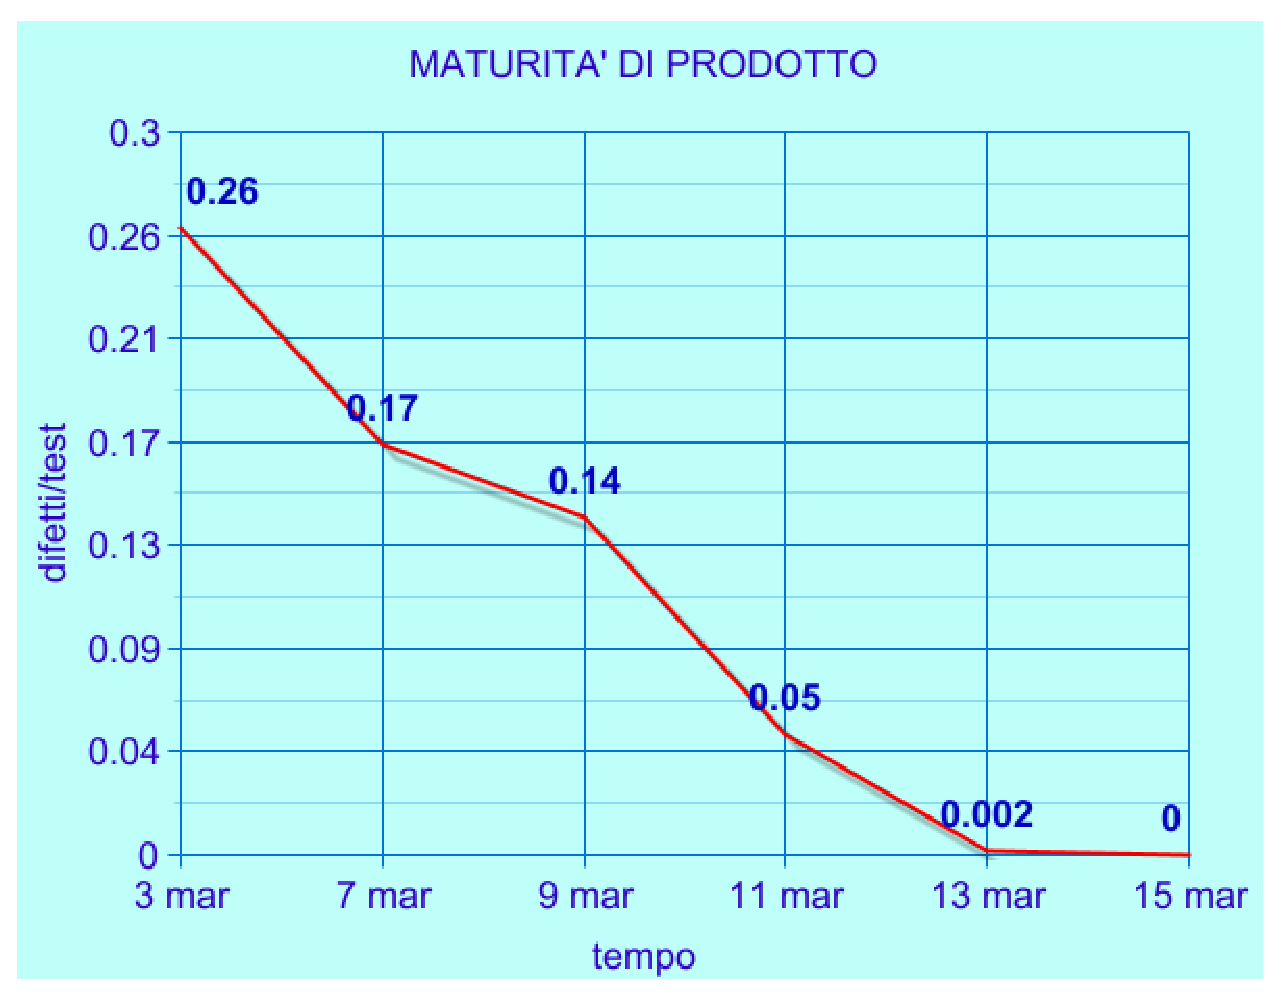
\includegraphics[width=1\textwidth] {MaturitaDiProdotto.eps}
\end{center}
\end{document}
